\usetikzlibrary{calc}
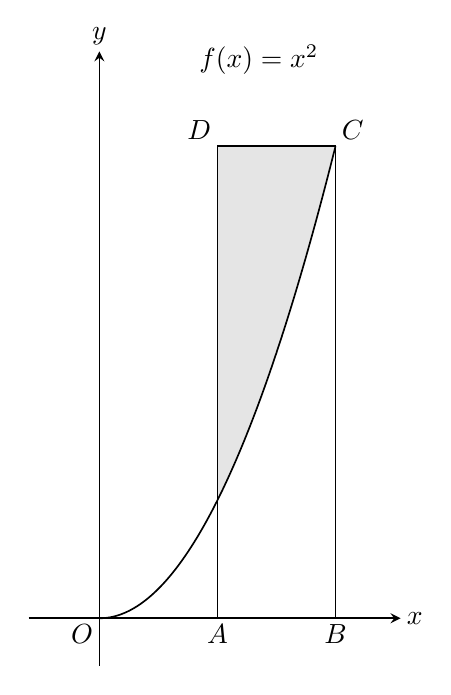
\begin{tikzpicture}[x=1.5cm,y=1.5cm,line width=.6pt,>=stealth,font=\normalsize]
\fill[gray!20] (1,4) -- (2,4) -- plot[domain=2:1,samples=80] (\x,{\x*\x}) -- cycle;
\draw[->] (-0.6,0) -- (2.55,0) node[right,inner sep=0pt,xshift=2pt] {$x$};
\draw[->] (0,-0.4) -- (0,4.8) node[above,inner sep=0pt,yshift=2pt] {$y$};
\draw (1,0) rectangle (2,4);
\draw[domain=0:2,samples=120] plot (\x,{\x*\x});
\node[below left,inner sep=0pt,xshift=-2pt,yshift=-2pt] at (0,0) {$O$};
\node[below,inner sep=0pt,yshift=-2pt] at (1,0) {$A$};
\node[below,inner sep=0pt,yshift=-2pt] at (2,0) {$B$};
\node[above left,inner sep=0pt,xshift=-2pt,yshift=2pt] at (1,4) {$D$};
\node[above right,inner sep=0pt,xshift=2pt,yshift=2pt] at (2,4) {$C$};
\node[above,inner sep=0pt,yshift=2pt] at (1.35,4.55) {$f(x)=x^{2}$};
\end{tikzpicture}
